\documentclass[11pt,twocolumn]{article}

\usepackage{graphicx}
\usepackage{textcomp}
\usepackage{cite}
\usepackage{hyperref}
\usepackage{multicol}
\usepackage{url}
\usepackage[margin=1in]{geometry}
\usepackage{amsmath,amssymb,amsthm, amsfonts, palatino, mathpazo, array}

\newcommand{\tab}[0] {\hspace*{24pt}}


\usepackage{graphicx}
\graphicspath{ {/home/ubuntu/www/octopress/source/} }

\usepackage{float}
\floatstyle{boxed} 
\restylefloat{figure}

\author{Andrew Gibiansky}
\def\title{Iranian Political Embargoes and Their Non-Existent Impact on Gasoline Prices}

\begin{document}

\subsection*{The Iranian Conflict}
\tab In the past several weeks, the media coverage of the rising gasoline prices has focused on the increasingly strained relationship between the western nations and Iran. For the past several years, the Iranian government has been striving to create purified uranium, with the stated intent of using solely for peaceful purposes, such as power generation\cite{1}. However, the potential for Iranian nuclear weapons has stirred the western governments into enforcing sanctions against Iran. The European Union has agreed to freeze assets of the Iranian central bank and to cease Iranian oil exports starting in July 2012; President Barack Obama decreed a freeze on assets and property belonging to Iranian financial institutions\cite{2}. Even although Obama has stated that he has no plans for strict sanctions against Iran, Congress has encouraged Obama to implement the harsher sanctions that it had approved previously\cite{4}. Even with western sanctions and embargoes, Iranian officials state that Iran has prepared for worst case scenarios and will continue work on uranium purification in Iran. In addition, Iran has responded to the European Union by ceasing the export of oil to other European countries, such as Britain and France\cite{3}.

\tab The political conflicts with Iran and the resulting oil embargo have created some public expectation of a supply-side crude oil shortage. Many market analysts and United States politicians have pinned the cause of rising gas prices to the western conflict with the Iranian government, citing a disruption in the supply of Iranian oil to the western world. Others state that the reason for the price rise is solely the result of rising tensions, rather than an effect of the reduced supply and demand. In particular, politicians believe this is a critical issue, because excessively high gasoline prices could hamper the economic recovery that Congress is hoping for. Obama has stated that instability in the Middle East (namely, in Iran) is the driving factor in recent price increases, although rising demand from China and speculative market trading are also factors. The Iranian conflict has led to increasing crude oil prices, and many believe that this, in turn, is pushing gasoline prices skyward. Before discussing the economics of the oil and gasoline markets, it is important to first understand gasoline and the process oil goes through to end up as gasoline in the tank of a consumer's car.

\subsection*{Gasoline Production}
\tab Gasoline is produced from petroleum (``crude oil''). Petroleum is a viscous, black liquid. It pools deep underground and is the result of organic matter being compressed and stored underground for millenia upon millenia, and high-tech pumps bring millions of barrels of it to the surface. Petroleum consists mostly of hydrocarbon chains of varying lengths. (A hydrocarbon chain is a sequence of carbon atoms bonded to each other, with hydrogen atoms pairing off with any remaining unpaired electrons.) Hydrocarbon chains come in different lengths; the lightest of them (methane through butane) only contain one to four carbon atoms, and are actually found as gasses at room temperature. These are available in natural gas, rather than petroleum. The next few chains, ranging from five to seven carbon atoms, are liquids at room temperature but evaporate quickly and are easily converted into gas form. Finally, gasoline is made from hydrocarbon chains with between seven and eleven carbon atoms. Kerosene and diesel are made from even longer hydrocarbon chains, and once they amass more than around twenty carbons, they begin to form solids and waxes instead of liquids. 

\tab After crude oil is extracted from the ground, it is shipped via container ship or pipeline to refineries. In order to create gasoline and other distillates from crude oil, oil refineries put the petroleum liquid through a process known as fractional distillation. The petroleum is heated to temperatures of up to 600° Celcius, at which point is is entirely vaporized; it is then allowed to cool. As the vapors cool, the heavier hydrocarbons condense at higher temperatures, while the lighter hydrocarbons condense at lower temperatures. Thus, the cooling of the gas allows refineries to separate the different types of hydrocarbons out of crude oil. In addition to separating types of hydrocarbons, oil refineries extract any impurities found in the oil, burn extra products for energy, and also break down longer hydrocarbon chains into shorter ones in order to produce more gasoline, diesel, or kerosene. 
\\\\
\subsection*{Gasoline Pricing}
\tab Gasoline is sold by a variety of local retailers and outlets; given the large number of sellers, classical supply and demand economics largely determine the price of gasoline. If the price of oil or other inputs gets lower (or the production or sale of gasoline in any way becomes cheaper), prices will be driven down, because franchises will be able to lower their prices in order to outperform their competitors; similarly, if production prices go up, prices will be pushed up. The large number of retailers will generally drive the market to some sort of equilibrium, although gas prices will vary by day and even by location. As one might expect, though, the equilibrium is determined by many factors, such as the price of crude oil. 

\tab Although gasoline prices are highly dependent upon crude oil prices, prices at the pump depend on a number of other things as well. In addition to the cost of buying crude oil, there is a cost associated with processing it and converting it into diesel, gasoline, and other useful materials, as well as an amortized cost for the construction of refineries and other elements of the supply chain. After accounting for the supply chain and production costs, state and local taxes apply to gasoline, and contribute to the difference in pricing between different regions. Similarly, different locales have different laws and regulations regarding gasoline purity and quality; there are at least eighteen different formulations of gasoline, and formulations are often restricted to only one or a few states where they may be sold.  Finally, gasoline distributors and retailers all take a cut of the profit, adding a retailer markup to the price consumers pay for gasoline. 
\begin{figure}
    \centering
    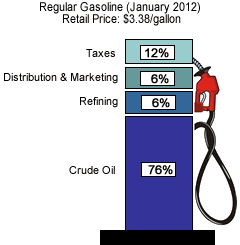
\includegraphics[scale=1.0]{images/GasolineDollarBreakdown.png}\\
A breakdown of gasoline prices by where the money goes. Taxes include federal,
state, and local taxes on gasoline. These proportions - particularly the
proportion due to crude oil costs - vary historically, but stay in roughly the
same range. However, they can fluctuate large amounts based on costs of
additives, the type and purity of the input crude oil, and how much distillates
are currently being imported and exported.
\end{figure}

\onecolumn
\begin{multicols}{2}
\subsection*{Futures Markets and Pricing Trends}
\tab Like many market-traded commodities, gasoline, diesel, and crude oil are all traded on international futures markets. The futures markets allow buyers and sellers to buy into or sell futures contracts. A futures contract is a contract promising the delivery or acceptance of some amount of a commodity; in simplest terms, a company may purchase a futures contract several months in advance, which will pay out the difference between the final spot price the company purchases at and the price which existed when the contract was purchased. For instance, if a company purchases a futures contract at \$100, and on the date of delivery the price had risen to \$120, the futures market ensures that the net amount of money the company must pay for the delivery is still only \$100. Although futures trading is a complicated matter, the point is that the prices quoted for oil and other commodities are actually the prices for futures contracts.

\tab In order to analyze recent changes in the price of crude oil and oil distillates, it is helpful to take a look at the historical trends in the price of crude oil. The U.S. Energy Information Administration (EIA) provides historical and current data for daily, monthly, or yearly spot prices. In order to make use of the provided historical prices, we must perform a moving average of our prices. This reduces the volatility of the prices and allows trends to show up more clearly, because the volatility due to noise is reduced by a wide moving average. In order to create a moving average, instead of using a data point, we use the data point averaged with several months worth of previous data points.
\end{multicols}

\begin{figure}
    \centering
    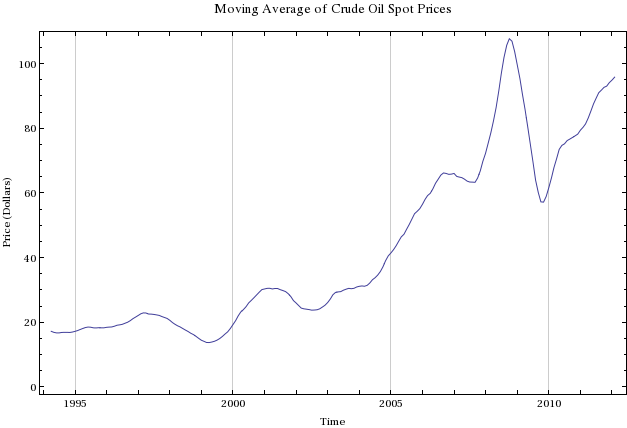
\includegraphics[scale=0.68]{images/CrudeMovingAverage.png}\\
    Moving averages of crude oil futures prices
\end{figure}
\newpage

\begin{figure}
    \centering
    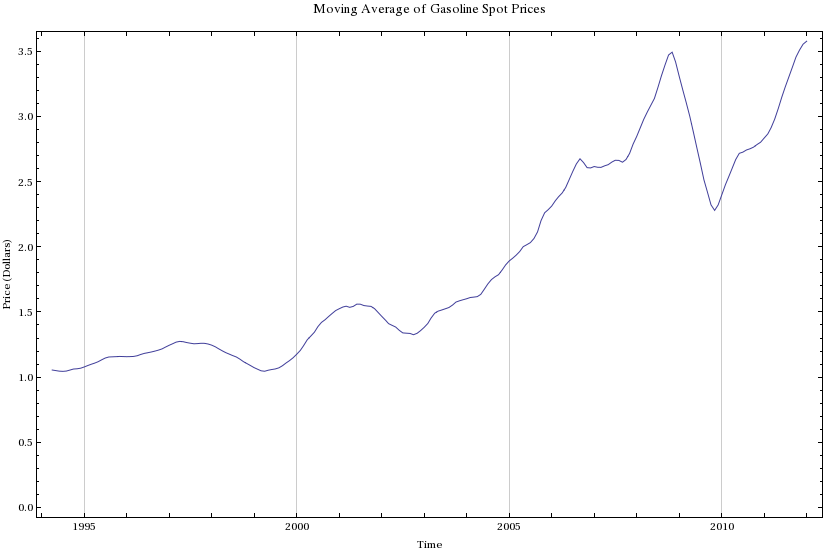
\includegraphics[scale=0.5]{images/GasolineMovingAverage.png}\\
    {Moving averages of gasoline futures prices}
\end{figure}

\begin{multicols}{2}
    \tab Graphing the twelve-month moving average of gasoline spot prices and WTI crude oil spot prices, we can immediately see – even just based on just purely visual inspection – that long-term gasoline prices follow crude oil prices pretty closely. In addition, we can see that although there are clearly blips and big events, such as the economic crash of the past decade (in which crude oil prices plunged), the prices of both gasoline and crude oil have been rising steadily and almost linearly for the most part. In general, both of these are more or less true; however, looking closer at individual regions of the graphs, we will see deviations.

    \tab If instead of graphing the past several years, we graph only the prices for this year (2012), we do indeed see a different picture. The graph of the price of crude oil seems to have little to no resemblance to the graph of gasoline prices. In the past several weeks, gasoline prices have been rising, and rising with an even greater speed past the beginning of February. However, oil prices were actually falling until early February, and started rising quite quickly around the beginning of February. We can, indeed, attribute this rise in oil prices to global events, such as the events in Iran; however, the rise in gasoline prices had been steady throughout the varying rate of change of oil prices. If the events in Iran had, in fact, caused gasoline prices to go up, we would have seen similar trends in the gasoline and oil prices, and gasoline prices would be noticeably affected by the increasing oil prices, and would start increasing even more rapidly once the prices of oil started going up. The fact that we do not see a clean relationship between oil prices and gasoline prices, and between the events in Iran and gasoline prices, implies that the Iranian situation had and has little or nothing to do with the rising gasoline prices.
\end{multicols}

\begin{figure}
    \centering
    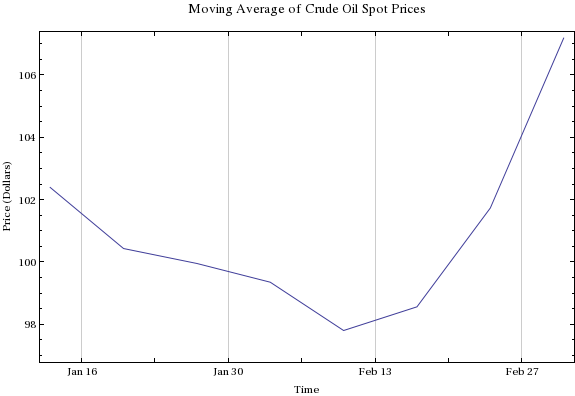
\includegraphics[scale=0.55]{images/RecentCrudePrices.png}\\
    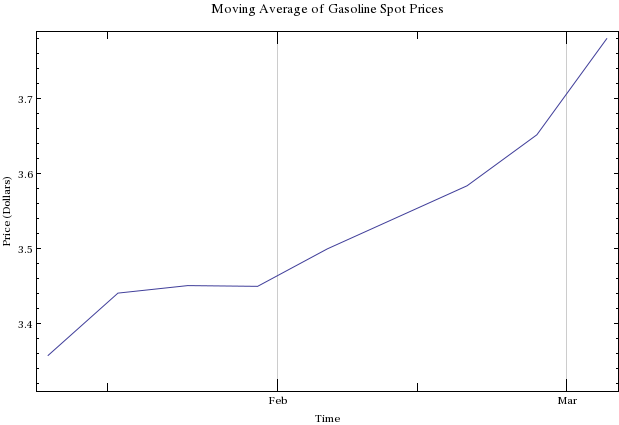
\includegraphics[scale=0.5]{images/RecentGasPrices.png} \\
    {Recent Crude Oil and Gasoline Spot Prices}
\end{figure}
\begin{multicols}{2}
\tab Although we expect a relationship when looking at recent price differentials in gasoline and crude oil, the relationship we are looking for is not perfectly straightforward. Although jumps in oil price manifest themselves as increases in gasoline spot prices, the rise in gasoline prices occurs after a time delay. Since crude oil bought on the futures market takes several weeks to transport to refineries and convert into gasoline, a time lag exists between the crude oil and gasoline spot prices, with crude oil changing first and later having an effect upon the gasoline prices. Thus, if there were an effect of Iranian events on gasoline prices, the effect would come significantly later than the events themselves; the Iranian situation deteriorated in late January after the European Union oil embargo, so we would not expect such events to influence gasoline prices until at least mid-February. However, we can see that the rise in gasoline prices begins before February, and continues through February without any significant change that could be attributed to Iranian political events. 

\subsection*{Rising Gasoline Prices}
\tab When looking for explanations for the steadily rising cost of gasoline, intuition immediately suggests that since the shapes of the crude oil price curve and the gasoline price curve, the gasoline price depends entirely upon the crude oil; however, there may be other factors at work. Of course, there is no way that gasoline could not depend on the price of crude oil, since between 50\% and 80\% of the price of gasoline is the cost of paying for the crude oil it is made of. If we assume that 65\% of the price of gasoline is used to pay for crude oil, as it has in recent years, a doubling in the price of crude oil will result in a 165\% increase in the price of gasoline. This gives us a mechanism by which we can check whether there are changes besides the change in the price of crude oil that are affecting the price of gasoline: since gasoline price is approximately 65\%  due to oil price, we expect that a five-fold increase in oil prices will result in a 3.6-fold increase in the price of gasoline. If 65\% of gasoline is due to oil prices, then 35\text{ cents}$\;$ per dollar is spent on other things; thus, if oil prices increase fivefold, gas that previously cost one dollar now costs
\[\text{New Cost} = 0.35\text{ cents} + 0.65\text{ cents}\times 5 = \$3.60.\]
\tab Over the course of the past twenty years, crude oil has gone from approximately \$20 per barrel to approximately \$105 per barrel, while gasoline has gone from approximately \$1 per gallon to \$3.7 per gallon. This is actually surprisingly close to what we would predict if we assumed that gasoline price changes are entirely determined by oil price changes, so we can reasonably assume that the most important factor in the change of oil prices for the past twenty years has been rising crude oil prices. \\
\tab Note that this estimation is \emph{incredibly} crude (no pun intended), and while it certainly cannot be used as predictive material, it is still indicative of the general trend.
\subsection*{Could Iran Have Influenced Oil Prices in the United States?}
In addition to the indicators discussed previously, there are a number of convincing reasons that the Iranian political crisis simply \emph{could not} have influenced United States gasoline prices. First of all, the United States oil imports from Iran are negligible to non-existent. In fact, the United States oil imported from the entire Middle East accounts for only approximately 15\% of U.S. crude oil imports - and of those 15\%, Iran supplies none of it. If the supply of United States crude oil is left unchanged by Iranian politics, the price of gasoline in the United States will be similarly unaffected. In addition to the unaffected supply, gasoline price changes will generally lag behind oil price changes by several weeks. Looking at the figure, we can see that the gasoline price change could not have possibly come from the change in oil price - simply because it would have to be lagged, whereas in the graph the gasoline prices begin to rise even \emph{before} oil prices. \\
\tab Given these data, there is no reason to rely upon the Iranian political situation for an explanation of the rising gas prices. The reasons behind the price increase can be explained adequately through other means. For instance, although it is not yet summer, we are quickly approaching May and June, and it is well-documented that proximity to the summer season will generally cause a price increase in the cost of gasoline. People will travel more often, some refineries will need to be shut down, etc; all of these contribute to rising gasoline prices that happen more or less annually. Although further explanation is beyond the scope of the paper, the gradual rise in gasoline prices is also affected by the increasing export levels of United States distillates, given the consistent refinery capacities throughout the past several decades.

\subsection*{Conclusion}
\tab Although gasoline prices seem to be influenced most by crude oil prices, it is unlikely that events in Iran have influenced gasoline prices in the last two months. Among other things, two major French and British oil importers (Total and BP, respectively) had already mostly ceased the import of Iranian oil, so the influence of recent events upon oil supply may be incredibly small; similarly, the United States does not import any crude oil from Iran. (In fact, only approximately one sixth of U.S. crude oil imports come from the Middle East at all.) In addition, the gasoline prices from the past month do not follow the crude oil prices; since the Iranian situation would only have a direct effect upon crude oil prices, the lack of a short-term relationship between crude oil and gasoline in the past month imply that the gasoline prices have been rising of their own accord, rather than due to Iranian political turmoil. Finally, a time lag is expected between crude oil price increases and gasoline price increases, so even if crude oil prices had increased due to Iranian events, the gasoline price increase was already well underway by the time these political happenings could begin to affect the price of gasoline; in fact, no noticeable change in the growth of gasoline prices exists. 

\tab We conclude that the increase in gasoline prices has little or nothing to due with the Western conflict with Iran, even though the steady increase in gasoline prices over the course of the past twenty years is almost completely due to the corresponding rise in crude oil prices.
\end{multicols}
\end{document}
